% Options for packages loaded elsewhere
\PassOptionsToPackage{unicode}{hyperref}
\PassOptionsToPackage{hyphens}{url}
\PassOptionsToPackage{dvipsnames,svgnames,x11names}{xcolor}
%
\documentclass[
  letterpaper,
  DIV=11,
  numbers=noendperiod]{scrreprt}

\usepackage{amsmath,amssymb}
\usepackage{iftex}
\ifPDFTeX
  \usepackage[T1]{fontenc}
  \usepackage[utf8]{inputenc}
  \usepackage{textcomp} % provide euro and other symbols
\else % if luatex or xetex
  \usepackage{unicode-math}
  \defaultfontfeatures{Scale=MatchLowercase}
  \defaultfontfeatures[\rmfamily]{Ligatures=TeX,Scale=1}
\fi
\usepackage{lmodern}
\ifPDFTeX\else  
    % xetex/luatex font selection
\fi
% Use upquote if available, for straight quotes in verbatim environments
\IfFileExists{upquote.sty}{\usepackage{upquote}}{}
\IfFileExists{microtype.sty}{% use microtype if available
  \usepackage[]{microtype}
  \UseMicrotypeSet[protrusion]{basicmath} % disable protrusion for tt fonts
}{}
\makeatletter
\@ifundefined{KOMAClassName}{% if non-KOMA class
  \IfFileExists{parskip.sty}{%
    \usepackage{parskip}
  }{% else
    \setlength{\parindent}{0pt}
    \setlength{\parskip}{6pt plus 2pt minus 1pt}}
}{% if KOMA class
  \KOMAoptions{parskip=half}}
\makeatother
\usepackage{xcolor}
\setlength{\emergencystretch}{3em} % prevent overfull lines
\setcounter{secnumdepth}{5}
% Make \paragraph and \subparagraph free-standing
\ifx\paragraph\undefined\else
  \let\oldparagraph\paragraph
  \renewcommand{\paragraph}[1]{\oldparagraph{#1}\mbox{}}
\fi
\ifx\subparagraph\undefined\else
  \let\oldsubparagraph\subparagraph
  \renewcommand{\subparagraph}[1]{\oldsubparagraph{#1}\mbox{}}
\fi


\providecommand{\tightlist}{%
  \setlength{\itemsep}{0pt}\setlength{\parskip}{0pt}}\usepackage{longtable,booktabs,array}
\usepackage{calc} % for calculating minipage widths
% Correct order of tables after \paragraph or \subparagraph
\usepackage{etoolbox}
\makeatletter
\patchcmd\longtable{\par}{\if@noskipsec\mbox{}\fi\par}{}{}
\makeatother
% Allow footnotes in longtable head/foot
\IfFileExists{footnotehyper.sty}{\usepackage{footnotehyper}}{\usepackage{footnote}}
\makesavenoteenv{longtable}
\usepackage{graphicx}
\makeatletter
\def\maxwidth{\ifdim\Gin@nat@width>\linewidth\linewidth\else\Gin@nat@width\fi}
\def\maxheight{\ifdim\Gin@nat@height>\textheight\textheight\else\Gin@nat@height\fi}
\makeatother
% Scale images if necessary, so that they will not overflow the page
% margins by default, and it is still possible to overwrite the defaults
% using explicit options in \includegraphics[width, height, ...]{}
\setkeys{Gin}{width=\maxwidth,height=\maxheight,keepaspectratio}
% Set default figure placement to htbp
\makeatletter
\def\fps@figure{htbp}
\makeatother
% definitions for citeproc citations
\NewDocumentCommand\citeproctext{}{}
\NewDocumentCommand\citeproc{mm}{%
  \begingroup\def\citeproctext{#2}\cite{#1}\endgroup}
\makeatletter
 % allow citations to break across lines
 \let\@cite@ofmt\@firstofone
 % avoid brackets around text for \cite:
 \def\@biblabel#1{}
 \def\@cite#1#2{{#1\if@tempswa , #2\fi}}
\makeatother
\newlength{\cslhangindent}
\setlength{\cslhangindent}{1.5em}
\newlength{\csllabelwidth}
\setlength{\csllabelwidth}{3em}
\newenvironment{CSLReferences}[2] % #1 hanging-indent, #2 entry-spacing
 {\begin{list}{}{%
  \setlength{\itemindent}{0pt}
  \setlength{\leftmargin}{0pt}
  \setlength{\parsep}{0pt}
  % turn on hanging indent if param 1 is 1
  \ifodd #1
   \setlength{\leftmargin}{\cslhangindent}
   \setlength{\itemindent}{-1\cslhangindent}
  \fi
  % set entry spacing
  \setlength{\itemsep}{#2\baselineskip}}}
 {\end{list}}
\usepackage{calc}
\newcommand{\CSLBlock}[1]{\hfill\break\parbox[t]{\linewidth}{\strut\ignorespaces#1\strut}}
\newcommand{\CSLLeftMargin}[1]{\parbox[t]{\csllabelwidth}{\strut#1\strut}}
\newcommand{\CSLRightInline}[1]{\parbox[t]{\linewidth - \csllabelwidth}{\strut#1\strut}}
\newcommand{\CSLIndent}[1]{\hspace{\cslhangindent}#1}

\KOMAoption{captions}{tableheading}
\makeatletter
\@ifpackageloaded{bookmark}{}{\usepackage{bookmark}}
\makeatother
\makeatletter
\@ifpackageloaded{caption}{}{\usepackage{caption}}
\AtBeginDocument{%
\ifdefined\contentsname
  \renewcommand*\contentsname{Table of contents}
\else
  \newcommand\contentsname{Table of contents}
\fi
\ifdefined\listfigurename
  \renewcommand*\listfigurename{List of Figures}
\else
  \newcommand\listfigurename{List of Figures}
\fi
\ifdefined\listtablename
  \renewcommand*\listtablename{List of Tables}
\else
  \newcommand\listtablename{List of Tables}
\fi
\ifdefined\figurename
  \renewcommand*\figurename{Figure}
\else
  \newcommand\figurename{Figure}
\fi
\ifdefined\tablename
  \renewcommand*\tablename{Table}
\else
  \newcommand\tablename{Table}
\fi
}
\@ifpackageloaded{float}{}{\usepackage{float}}
\floatstyle{ruled}
\@ifundefined{c@chapter}{\newfloat{codelisting}{h}{lop}}{\newfloat{codelisting}{h}{lop}[chapter]}
\floatname{codelisting}{Listing}
\newcommand*\listoflistings{\listof{codelisting}{List of Listings}}
\makeatother
\makeatletter
\makeatother
\makeatletter
\@ifpackageloaded{caption}{}{\usepackage{caption}}
\@ifpackageloaded{subcaption}{}{\usepackage{subcaption}}
\makeatother
\ifLuaTeX
  \usepackage{selnolig}  % disable illegal ligatures
\fi
\usepackage{bookmark}

\IfFileExists{xurl.sty}{\usepackage{xurl}}{} % add URL line breaks if available
\urlstyle{same} % disable monospaced font for URLs
\hypersetup{
  pdftitle={Electromagnetism},
  pdfauthor={Claire Greenland},
  colorlinks=true,
  linkcolor={blue},
  filecolor={Maroon},
  citecolor={Blue},
  urlcolor={Blue},
  pdfcreator={LaTeX via pandoc}}

\title{Electromagnetism}
\author{Claire Greenland}
\date{2024-03-25}

\begin{document}
\maketitle

\renewcommand*\contentsname{Table of contents}
{
\hypersetup{linkcolor=}
\setcounter{tocdepth}{2}
\tableofcontents
}
\bookmarksetup{startatroot}

\chapter*{Preface}\label{preface}
\addcontentsline{toc}{chapter}{Preface}

\markboth{Preface}{Preface}

\newcommand{\l}{\mathrm{\mathbf{l}}}
\newcommand{\E}{\mathrm{\mathbf{E}}}
\newcommand{\F}{\mathrm{\mathbf{F}}}
\newcommand{\r}{\mathrm{\mathbf{r}}}

\newcommand{\x}{\mathrm{\mathbf{x}}}
\newcommand{\y}{\mathrm{\mathbf{y}}}
\newcommand{\z}{\mathrm{\mathbf{z}}}

This is a Quarto book.

To learn more about Quarto books visit
\url{https://quarto.org/docs/books}.

Put a nice introduction here introducing the subject of electromagnetism
:D

\bookmarksetup{startatroot}

\chapter{Electrostatics - Charges, Forces \&
Fields}\label{electrostatics---charges-forces-fields}

\newcommand{\l}{\mathrm{\mathbf{l}}}
\newcommand{\E}{\mathrm{\mathbf{E}}}
\newcommand{\F}{\mathrm{\mathbf{F}}}
\newcommand{\r}{\mathrm{\mathbf{r}}}

\newcommand{\x}{\mathrm{\mathbf{x}}}
\newcommand{\y}{\mathrm{\mathbf{y}}}
\newcommand{\z}{\mathrm{\mathbf{z}}}

\emph{Recommended reading}: Griffiths Section 2.1 (and 2.2 if you want
some bonus reading about stuff that will be important later)

\section{Pre-lecture problem}\label{pre-lecture-problem}

Griffiths Problem 1.7

\section{Electric Charges}\label{electric-charges}

Electric charge is a fundamental property of matter. Many fundamental
particles (such as electrons and protons) have charge. However,
macroscopic objects can also be charged due to having a distribution of
charged particles on them that has a small imbalance in charge - we
might describe these as ``charged objects''.

Charge gives rise to electric fields, and hence to the electric forces
experienced between charged particles or objects.

Charge can be either a positive or negative quantity. ``Like'' charges
(charges with the same sign) repel each other, and opposite charges
attract.

Charge is quantized and comes in integer multiples of the elementary
charge \(e\) which has an approximate value of
\(1.602 \times 10 ^{-19}\) Coulombs. Electrons carry a charge of \(-e\),
and protons carry a charge of \(+e\). Charges measured in laboratories
are always multiples of \(e\) but the quarks inside protons and neutrons
and other hadrons have charges that are fractions of this elementary
charge.

Charge is conserved - or more specifically, the total charge in an
isolated system is conserved. (At least, this has been the case in all
the particle interactions physicists have so far observed.) Hence,
charge can be neither created nor destroyed, but can only be transferred
from one object to another.

\textbf{Gravitational charge:} there is one type of gravitational
charge, which is mass/energy. Gravitational charges attract. We don't
know about quantization of mass. (You can probably spend many hours on
the internet reading different opinions on this). Mass/Energy is
conserved and all everyday objects are gravitationally charged so they
all attract each other, but gravity is very weak--we can easily pick up
bits of paper with an electrically charged rod when rather few electrons
have been moved.

\section{Some definitions and important
notation}\label{some-definitions-and-important-notation}

Here I will briefly explain some notation and definitions I will use in
this course for setting up and solving problems involving electric
charges.

Consider the following ensemble of charges:

\begin{figure}[H]

{\centering 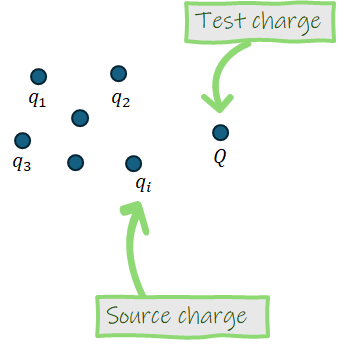
\includegraphics{Figures/sourcetest_definitions.png}

}

\caption{Some charges.}

\end{figure}%

We define the charges \(q_1\), \(q_2\), \(q_3\)\ldots{} \(q_i\) as
source charges, meaning that these are the charges that produce the
electric field for the purpose of the problem. We define \(Q\) as the
test charge, which means it is the charge that is experiencing the
effects of the electric field produced by the source charge(s). It is
important to note that any charge can be a source or a test charge,
there is no fundamental difference between them. ``Source'' and ``test''
are simply names that we give charges when setting up a problem, so that
we can more easily define and solve the problem.

Throughout this course you will also see the terms ``source point'' and
``field point''. The source point is the location of the source
charge(s), while the field point is essentially the location of the test
charge. If there is no test charge in the problem (for example if we are
computing the electric field of a source charge), the field point is the
point at which we are measuring the field - it is the point where a test
charge would be if there was one.

\begin{figure}[H]

{\centering 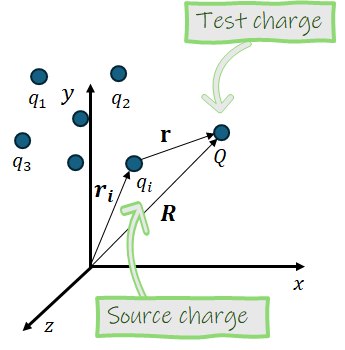
\includegraphics{Figures/axes_r_definitions.png}

}

\caption{Some charges, overlaid with axes showing the definition of
\(\mathrm{\mathbf{r}}\), the vector separation between the source and
test charges.}

\end{figure}%

\section{Electric Forces \& Coulomb's
Law}\label{electric-forces-coulombs-law}

All charges produce electric fields, and other charges that are in the
prescence of this field experience a force as a result.

The force on a test charge \(Q\), exerted by a source charge \(q\), is
given by Coulomb's Law, which is as follows:
\[ F = \frac{1}{4\pi \epsilon_0} \frac{q Q}{r_s^2} \hat{\mathrm{\mathbf{r}}_s} \]

where:

\begin{itemize}
\tightlist
\item
  \(\hat{\mathrm{\mathbf{r}}}\) is the unit vector in the direction of
  the force, which points from \(q\) to \(Q\).
\item
  \(r\) is the separation between \(q\) and \(Q\).
\item
  \(\epsilon_0\) is a physical constant known as the
  \bf{permittivity of free space}.  $\epsilon_0 \approx 8.85 \times 10^{-12}$ Fm $^{-1}$ (farads per metre). 
\end{itemize}

If \(q\) and \(Q\) have the same sign (like charges) the force is
repulsive (\(\mathrm{\mathbf{F}}\) is a positive quantity); if \(q\) and
\(Q\) have different signs, the force is attractive
(\(\mathrm{\mathbf{F}}\) is a negative quantity).

\section{Electric Field}\label{electric-field}

The electric field \(\mathrm{\mathbf{E}}\) produced by a charge (or
charged object/charge distribution) is a vector field that represents
the force per unit charge experienced by a positive test charge placed
at a particular point in space:

\[ \mathrm{\mathbf{E}}= \frac{\mathrm{\mathbf{F}}}{Q} \]

\noindent which can be rearranged to the more familiar form
\(\mathrm{\mathbf{F}}= Q \mathrm{\mathbf{E}}\).

\(\mathbf{E}\) has units of Vm\(^{-1}\) or NC\(^{-1}\).

The electric field is normally represented by field lines that indicate
the direction of the field. The direction of the field is determined by
what a positive test charge will do. That's why field lines point
towards negative charges - that's the direction a positive charge would
travel if it encountered the field of a negative charge. The density of
lines/arrows indicates the strength of the field at a point. You may
also see fields drawn where the size of the arrows represents the
electric field strength. The diagram below shows the electric field
lines for two positive point charges of the same magnitude.

\begin{figure}[H]

{\centering 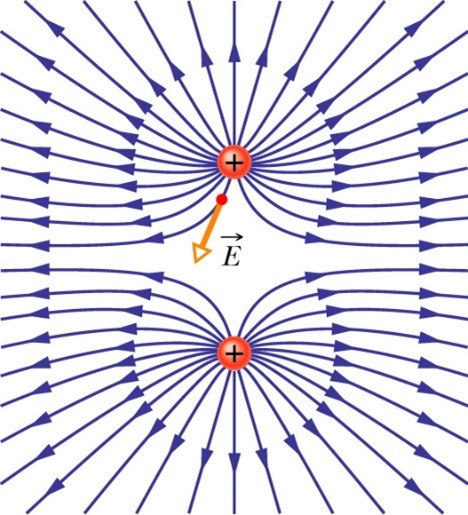
\includegraphics{Figures/Efield_like.png}

}

\caption{Representation of the electric field surrounding two positive
charges.}

\end{figure}%

Most important rules for field lines:

\begin{itemize}
\item
  Lines begin on positive charges and end on negative charges.
\item
  Lines never intersect.
\item
  Lines are symmetric as they leave the charges.
\end{itemize}

\section{Superposition Principle}\label{superposition-principle}

The principle of superposition states that ``the interaction between any
two charges is completely unaffected by the presence of others''. This
means that the total force on a test charge can be computed by
calculating the force on the test charge due to each source charge
separately, then adding up the contributions, as follows:

\[ \mathrm{\mathbf{F}}_{tot} = \sum_i \mathrm{\mathbf{F}}_i \]

The same applies to the electric field, which can be calculated for any
given point in space as a sum of the electric field at that point from
all the source charges:
\[ \mathrm{\mathbf{E}}_{tot} = \sum_i \mathrm{\mathbf{E}}_i \]

\section{Summary}\label{summary}

Electric charges create electric fields, which exert forces on other
charges. Coulomb's Law describes the force between point charges.

\section{Bonus content: vector
fields}\label{bonus-content-vector-fields}

\subsection{What is a field?}\label{what-is-a-field}

\emph{Recommended reading:}

A field is a region of space, where property of that space is
characterized by either a number (a scalar field) or by three numbers (a
vector field).

The concept of a field circumvents the problem of action at a distance,
where one inanimate object is ``aware'' that another has arrived. We
understand that the first body sets up a field and the second body
interacts with the first via this field.

\subsection{Scalar and vector fields}\label{scalar-and-vector-fields}

A scalar field is characterized at each point by a single number.
e.g.~the temperature, \(T\), at each position in a block of metal heated
at some places and cooled at others.

\begin{figure}[H]

{\centering 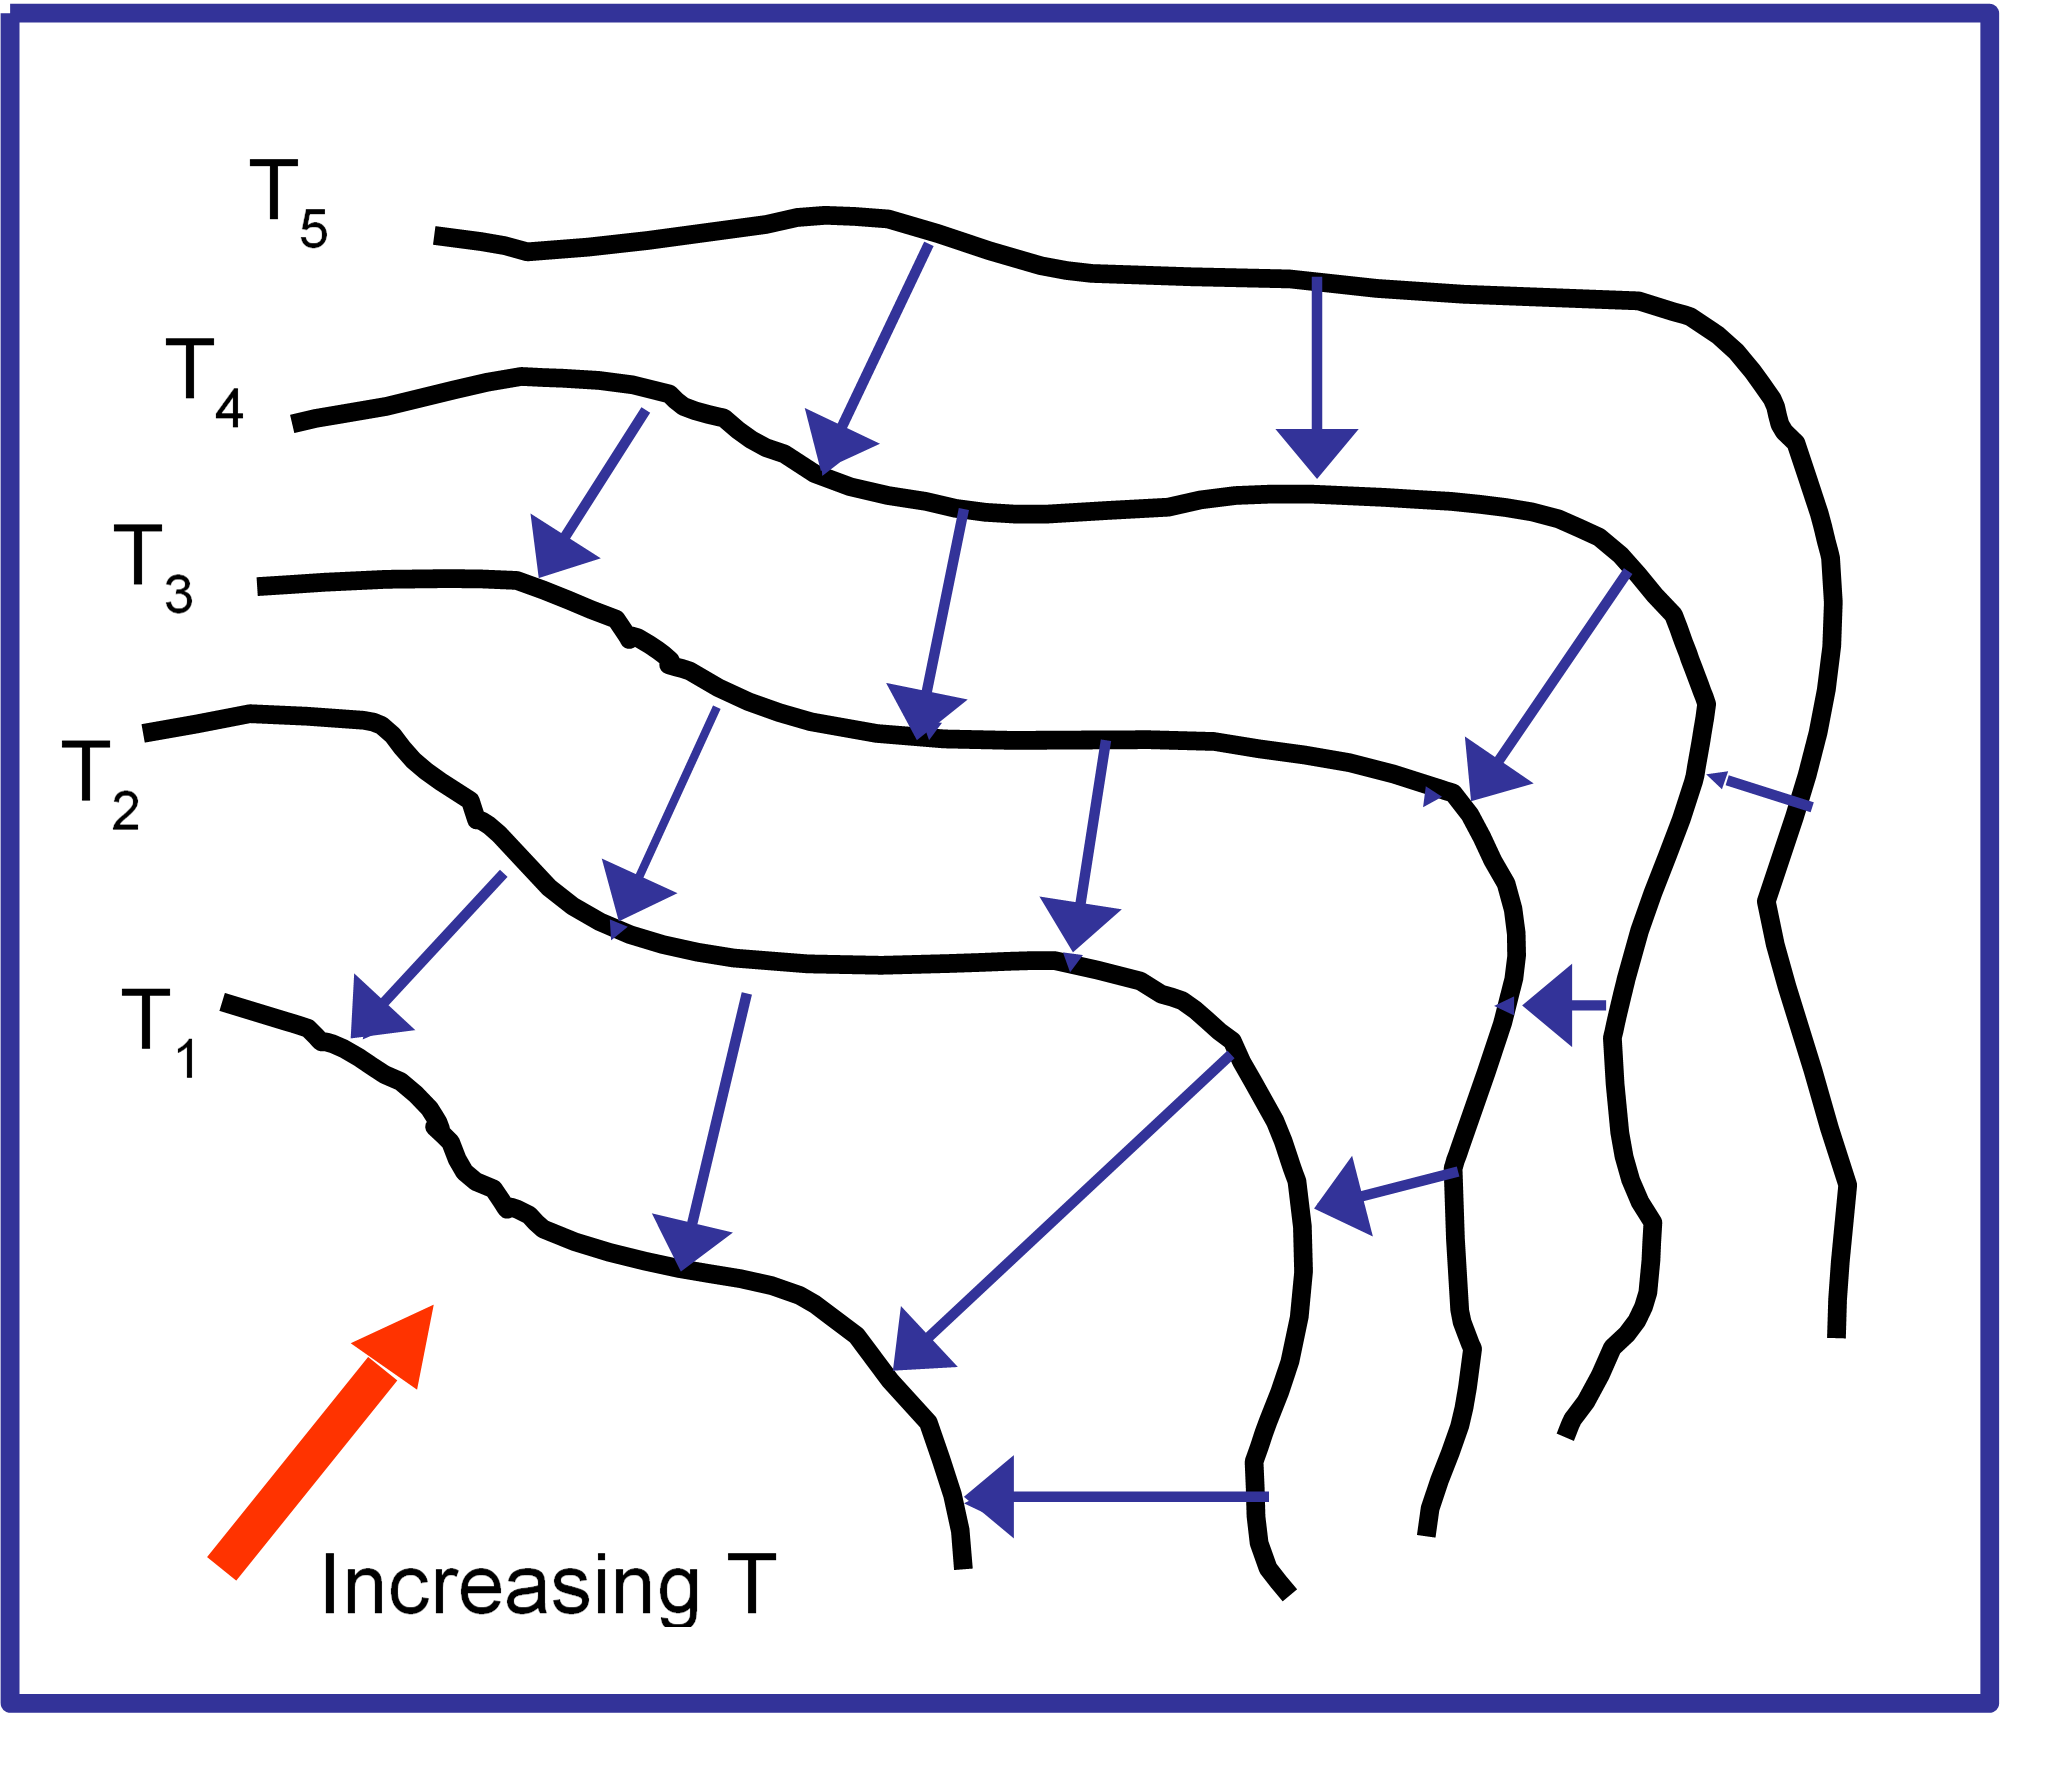
\includegraphics[width=80mm,height=\textheight]{Figures/isotherms.png}

}

\caption{A representation of a temperature field. Isotherms at different
temperatures are black lines; blue arrows show the direction of heat
flow, which is always perpendicular to the isotherms.}

\end{figure}%

\(T\) is a function of position i.e.~\(T = T(x,y,z)\). At every point we
can measure the scalar value of the temperature \(T\). The black lines
represent isotherms i.e.~lines where the temperature is constant
(\(T_1 < T_2 < T_3 < T_4 < T_5\)). Heat flow (blue arrows) is
perpendicular to the contours of constant temperature - the isotherms
(\(T_1\), \(T_2\) etc). The magnitude of the heat flow is proportional
to the temperature gradient, so that the heat flow is larger when
isotherms are closer together.

The scalar temperature field has an associated vector field, because at
any point, the heat flow is a vector, the \textbf{magnitude} and
\textbf{direction} of which depend on position. Heat flow is therefore a
vector field which is related to the scalar field of temperature. The
vector gradient of the field of heat flow depends on the temperature at
each point.

\subsection{Link between scalar and vector
field}\label{link-between-scalar-and-vector-field}

\emph{Recommended reading:}

For the scalar temperature field \(T(x,y,z)\) the vector describing the
direction and the magnitude of the maximum temperature gradient is:

\begin{equation}
 \text{Grad} \; T = \nabla T = \frac{\partial T} {\partial x} \hat{\mathbf{i}} + \frac{\partial T}{\partial y} \hat{\mathbf{j}} + \frac{\partial T}{\partial y} \hat{\mathbf{k}}
\end{equation}

The heat flow is a vector given by \(\mathbf{Q} = -k \nabla T\); the
minus sign is because heat flows from high temperature to low
temperature.

In general, for a scalar potential
\(-\nabla \phi = \frac{\partial \phi} {\partial x} \hat{\mathbf{i}} + \frac{\partial \phi}{\partial y} \hat{\mathbf{j}} + \frac{\partial \phi}{\partial y} \hat{\mathbf{k}}\)
describes the magnitude and direction of the physical effects of the
potential, with an appropriate constant if needed. In the case of the
electric field if the electric potential is \(V\) then the vector field
\(\mathbf{E} = -\nabla V\).

As an example, the gravitational field can be obtained from the
gravitational potential. The scalar gravitational potential energy is
given by \(U = mgz\) near the Earth's surface, where \(z\) is the
height. The gravitational potential is \(U/m = gz\). The gravitational
field is \(-\nabla(gz)=-g \hat{\mathbf{k}}\).

\subsection{Other operations on
vectors}\label{other-operations-on-vectors}

The vector operator \(\nabla\) behaves as a vector. We have looked at
grad \(\nabla\phi\) where \(\phi\) is a scalar field. In Maxwell's
equations, which you cover next year, you will also meet \(\nabla\)
operating on the electric field \(\mathbf{E}\):

\(\nabla \cdot \mathbf{E}\) (div or divergence)

\(\nabla \times \mathbf{E}\) (curl or rotation)

Maxwell's equations are one of the great achievements of 19th century
Physics. They link the phenomena of electricity and magnetism and can be
used to derive an expression for the speed of light. Einstein said that
the theory of Relativity was rooted in Maxwell's equations. The
equations in their differential form are shown below and we will meet
most of the concepts in this course and integral versions of some of the
laws. You can read more about Maxwell's Equations in Chapter 30 of
Tipler and Mosca.

\begin{equation}

\nabla \cdot \mathbf{E} = \frac{\rho}{\epsilon_0}
\end{equation}

\begin{equation}
\nabla \times \mathbf{E} = - \frac{\partial \mathbf{B}}{\partial t} 
\end{equation}

\begin{equation}
\nabla \cdot \mathbf{B} = 0
\end{equation}

\begin{equation}
\nabla \times \mathbf{B} = \frac{\mathbf{j}}{c^2 \epsilon_0} + \frac{1}{c^2} \frac{\partial \mathbf{E}}{\partial t}
\end{equation}

Source:
\url{http://www.clerkmaxwellfoundation.org/html/about_maxwell.html} ;
\url{https://maxwells-equations.com/}

\section{Post-lecture problem}\label{post-lecture-problem}

In the lecture, we found the electric field (magnitude and direction) a
distance \(z\) above the midpoint between two equal charges, \(q\), a
distance \(d\) apart. We found that for distances \(z\)
\textgreater\textgreater{} \(a\), as we might expect the field appears
like that of a single charge \(2q\).

\textbf{Q:} Repeat the calculation of the electric field, but replace
one of the positive charges with a negative charge (so we now have a
dipole). Is there anything interesting about this result {[}hint: try
computing the field for different ranges of \(z\)-values{]}?

\bookmarksetup{startatroot}

\chapter{Electric Potential}\label{electric-potential}

\newcommand{\l}{\mathrm{\mathbf{l}}}
\newcommand{\E}{\mathrm{\mathbf{E}}}
\newcommand{\F}{\mathrm{\mathbf{F}}}
\newcommand{\r}{\mathrm{\mathbf{r}}}

\newcommand{\x}{\mathrm{\mathbf{x}}}
\newcommand{\y}{\mathrm{\mathbf{y}}}
\newcommand{\z}{\mathrm{\mathbf{z}}}

\newcommand{\a}{\mathrm{\mathbf{a}}}
\newcommand{\b}{\mathrm{\mathbf{b}}}

\emph{Recommended reading}: Griffiths Section 2.3

\section{Pre-lecture problem}\label{pre-lecture-problem-1}

One of these is an impossible electrostatic field. Which one?

\begin{enumerate}
\def\labelenumi{(\alph{enumi})}
\item
  \$ \mathrm{\mathbf{E}} = k{[}xy \hat{\mathrm{\mathbf{x}}} +
  2yz\hat{\mathrm{\mathbf{y}}} + 3xz \hat{\mathrm{\mathbf{z}}} {]} \$
\item
  \$ \mathrm{\mathbf{E}} = k{[}y\^{}2 \hat{\mathrm{\mathbf{x}}} + (2xy +
  z\^{}2)\hat{\mathrm{\mathbf{y}}} + 2yz \hat{\mathrm{\mathbf{z}}} {]}\$
\end{enumerate}

\section{Introduction to electric
potential}\label{introduction-to-electric-potential}

Electric potential is a scalar quantity associated with the electric
field. It is defined as the work done by an external force to bring a
unit positive charge to a particular point in space (for example, at the
location of a test charge \(Q\)) from an arbitrary reference point. For
the purposes of this lecture course, we will choose infinity
(\(\infty\)) as our reference point - but please note that Griffiths
does not use infinity but rather uses the symbol \(\mathcal{O}\) to
denote an arbitrary reference point.

We will see later how the concept of electric potential simplifies many
calculations in electrostatics, particularly when dealing with electric
fields and potential energy.

\section{Definition of Electric
Potential}\label{definition-of-electric-potential}

The electric potential \(V\) at some displacement
\(\mathrm{\mathbf{r}}\) is given by

\$\$

V(\mathrm{\mathbf{r}}) = −\int\_\{\infty\}\^{}r
\mathrm{\mathbf{E}} \cdot \mathrm{d}\mathrm{\mathbf{l}} 

\$\$

where \(\mathrm{\mathbf{E}}\) is the electric field, and
\(\mathrm{d}\mathrm{\mathbf{l}}\) is an infinitesimal displacement
vector along the path of the charge. As we have stated, the potential is
the work done per unit charge, therefore we can see how the above can be
derived. The work done by a force to bring an object from infinity to
point \(\mathrm{\mathbf{r}}\) is given by \$ \int\emph{\infty\^{}r
\mathrm{\mathbf{F}} \cdot \mathrm{d}\mathrm{\mathbf{l}}\$, therefore the
work done per unit charge is \$\int}\infty\^{}r
\frac{\mathrm{\mathbf{F}}}{Q} \cdot \mathrm{d}\mathrm{\mathbf{l}} =
\int\emph{\infty\^{}r
\mathrm{\mathbf{E}} \cdot \mathrm{d}\mathrm{\mathbf{l}} \$. However, you
will notice that the expression shown above is \$ - \int}\infty\^{}r
\mathrm{\mathbf{E}} \cdot \mathrm{d}\mathrm{\mathbf{l}} \$ - by
convention, we add a minus sign because the direction of the electric
field is the direction of \emph{decreasing} potential. Let me explain
this. We have seen in the previous lecture that electric field lines
point away from a positive charge. If we place a positive test charge in
the vicinity of another positive charge, the test charge will move away,
in the direction of the electric field. This is the direction of
decreasing potential because the charge loses potential energy as it
moves away. Hence, the electric field points in the direction of
decreasing potential, so the expression for potential must be the
negative of the electric field.

\section{Potential Difference}\label{potential-difference}

The potential difference \(V_{ab}\) between two points
\(\mathrm{\mathbf{a}}\) and \(\mathrm{\mathbf{b}}\) is given by:

\$\$

V\_\{ab\} = V(\mathrm{\mathbf{b}}) − V(\mathrm{\mathbf{a}}) =
-\int\emph{\{\infty\}\^{}\{\mathrm{\mathbf{b}}\}
\mathrm{\mathbf{E}} \cdot \mathrm{d} \mathrm{\mathbf{l}} +
\int}\{\infty\}\^{}\{\mathrm{\mathbf{a}}\}
\mathrm{\mathbf{E}} \cdot \mathrm{d} \mathrm{\mathbf{l}} =
-\int\emph{\{\infty\}\^{}\{\mathrm{\mathbf{b}}\}
\mathrm{\mathbf{E}} \cdot \mathrm{d} \mathrm{\mathbf{l}} -
\int}\{\mathrm{\mathbf{a}}\}\^{}\{\infty\}
\mathrm{\mathbf{E}} \cdot \mathrm{d} \mathrm{\mathbf{l}} =
-\int\_\{\mathrm{\mathbf{a}}\}\^{}\{\mathrm{\mathbf{b}}\}
\mathrm{\mathbf{E}} \cdot \mathrm{d} \mathrm{\mathbf{l}}

\$\$

\$\$

V\_\{ab\} = V(\mathrm{\mathbf{b}}) − V(\mathrm{\mathbf{a}}) =
-\int\_\{\mathrm{\mathbf{a}}\}\^{}\{\mathrm{\mathbf{b}}\}
\mathrm{\mathbf{E}} \cdot \mathrm{d} \mathrm{\mathbf{l}} 

\$\$

This quantity represents the work done per unit charge by the electric
field in moving a charge from point \(\mathrm{\mathbf{a}}\) to point
\(\mathrm{\mathbf{b}}\).

\section{Electric Potential Due to a Point
Charge}\label{electric-potential-due-to-a-point-charge}

For a point charge \(q\) located at the origin, the electric potential
at a displacement \(\mathrm{\mathbf{r}}\) can be found by computing the
potential difference between infinity and the point
\(\mathrm{\mathbf{r}}\) - that is, the work done per unit charge in
bringing a test charge from infinity to point \(\mathrm{\mathbf{r}}\).
Try using the expression for \(V_{AB}\) above to do this - you can use
\(\mathrm{d}\mathrm{\mathbf{r}}\) as the displacement vector
\(\mathrm{d}\mathrm{\mathbf{l}}\). You should find that the potential
due to a point charge is therefore:

\$\$

V(\mathrm{\mathbf{r}}) = \frac{1}{4\pi\epsilon_0}
\frac{q}{\mathrm{\mathbf{r}}}

\$\$

\section{Electric Potential Due to Multiple Point
Charges}\label{electric-potential-due-to-multiple-point-charges}

The principle of superposition applies to electric potential, just as it
does to electric fields and forces. For multiple point charges \(q_i\)
located at positions \(\mathrm{\mathbf{r}}_i\), the total potential at a
point \mathrm{\mathbf{r}}is the sum of the potentials due to each
charge:

\$\$

V(r) = \frac{1}{4\pi \epsilon_0} \sum\_\{i\}
\frac{q_i}{|\mathrm{\mathbf{r}}- \mathrm{\mathbf{r}}_i|} \$\$

\section{Relationship Between Electric Field and Potential (Poisson's
and Laplace's
equation)}\label{relationship-between-electric-field-and-potential-poissons-and-laplaces-equation}

The electric field is related to the electric potential by the gradient:
\(\mathrm{\mathbf{E}}= -\nabla V\). This relationship implies that the
electric field points in the direction of the greatest decrease of
potential.

\section{Potential of a continuous charge
distribution}\label{potential-of-a-continuous-charge-distribution}

\section{Equipotential Surfaces}\label{equipotential-surfaces}

Equipotential surfaces are surfaces on which the electric potential is
constant. No work is required to move a charge along an equipotential
surface, because work is only required to change an object's potential.
Electric field lines are always perpendicular to equipotential surfaces.

\section{Example 1: Potential of a uniformly charged
sphere}\label{example-1-potential-of-a-uniformly-charged-sphere}

For a continuous charge distribution with volume charge density
\(\rho(\mathrm{\mathbf{r}}')\), the electric potential at a point
\(\mathbf{r}\) is: V(r)=ke∫ρ(r′)∣r−r′∣d3r′V(\mathbf{r}) = k\_e
\int \frac{\rho(\mathbf{r'})}{|\mathbf{r} - \mathbf{r'}|}
d\^{}3\mathbf{r'}V(r)=ke∫∣r−r′∣ρ(r′)d3r′

\section{Summary}\label{summary-1}

Electric potential is a crucial concept in electrostatics, simplifying
the analysis of electric fields and the work done by (or on) charges. It
is \textasciitilde intimately related\textasciitilde?? to the electric
field and provides a scalar measure of potential energy per unit charge.
Understanding electric potential is essential for solving a wide range
of problems in electrostatics.

\section{Post-lecture problem}\label{post-lecture-problem-1}

In the pre-lecture problem, hopefully you had a think about how we might
go about finding out which of the following two functions is an
impossible one.

\textbf{Q:} For the \emph{possible} one, find the potential. Use the
origin as your reference point. Check your answer by computing
\(\nabla V\).

{[}Hint: you must select a specific path to integrate along. The answer
is \textbf{path-independent}, meaning that you will get the same answer
no matter what path you choose--however, it is simply not possible to
integrate unless you have a particular path in mind.{]}

\bookmarksetup{startatroot}

\chapter{Work and Energy in
Electrostatics}\label{work-and-energy-in-electrostatics}

\newcommand{\l}{\mathrm{\mathbf{l}}}
\newcommand{\E}{\mathrm{\mathbf{E}}}
\newcommand{\F}{\mathrm{\mathbf{F}}}
\newcommand{\r}{\mathrm{\mathbf{r}}}

\newcommand{\x}{\mathrm{\mathbf{x}}}
\newcommand{\y}{\mathrm{\mathbf{y}}}
\newcommand{\z}{\mathrm{\mathbf{z}}}
\newcommand{\p}{\mathrm{\mathbf{p}}}
\newcommand{\d}{\mathrm{\mathbf{d}}}

\newcommand{\a}{\mathrm{\mathbf{a}}}
\newcommand{\b}{\mathrm{\mathbf{b}}}

\emph{Recommended reading}: Griffiths Section 2.4

\section{Work done to move a charge}\label{work-done-to-move-a-charge}

In general, the work done to move an electric charge is calculated in
the same way we calculate mechanical work when solving mechanics
problems, taking the form:

\$\$

W = \int \mathrm{\mathbf{F}} \cdot \mathrm{d} \mathrm{\mathbf{l}} 

\$\$

Let's say we have some configuration of source charges, and we want to
move a test charge past these charges, as represented in this diagram:

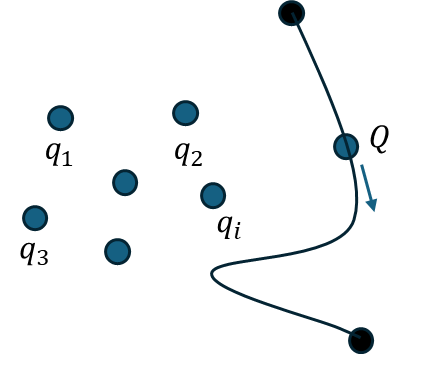
\includegraphics[width=3.125in,height=\textheight]{Figures/workdone_charge.png}

Let us work out how much work we need to do to move the charge along
this path. The work done to move a charge from point \textbf{a} to point
\textbf{b} is given by:

\$\$

W = \int\_\{\mathrm{\mathbf{b}}\}\^{}\{\mathrm{\mathbf{a}}\}
\mathrm{\mathbf{F}} \cdot \mathrm{d} \mathrm{\mathbf{l}} 

\$\$

Each of the charges is exerting a force
\(\mathrm{\mathbf{F}}= Q \mathrm{\mathbf{E}}\) on the test charge,
therefore the total work becomes:

\$\$

W = - Q \int\_\{\mathrm{\mathbf{b}}\}\^{}\{\mathrm{\mathbf{a}}\}
\mathrm{\mathbf{E}} \cdot \mathrm{d} \mathrm{\mathbf{l}} =
Q{[}V(\mathrm{\mathbf{b}}) - V(\mathrm{\mathbf{a}}){]}

\$\$

This equation re-states what we discussed in Lecture 2 - that the
potential difference between two points \(\mathrm{\mathbf{a}}\) and
\(\mathrm{\mathbf{b}}\) is the work done per unit charge to bring a
charge from point \(\mathrm{\mathbf{a}}\) to point
\(\mathrm{\mathbf{b}}\).

\section{Energy of a point charge
distribution}\label{energy-of-a-point-charge-distribution}

\section{Energy of a continuous charge
distribution}\label{energy-of-a-continuous-charge-distribution}

\begin{enumerate}
\def\labelenumi{\arabic{enumi}.}
\setcounter{enumi}{9}
\item
  Work and Energy in Electrostatics The work done to assemble a system
  of charges is related to the potential energy stored in the system.
  For point charges, the electrostatic potential energy \(U\) is given
  by:
\item
  Energy Density of the Electric Field
\end{enumerate}

The energy density uuu of the electric field is: u=12ϵ0E2u = \frac{1}{2}
\epsilon\_0 E\^{}2u=21ϵ0E2 where ϵ0\epsilon\_0ϵ0 is the permittivity of
free space. The total electrostatic energy stored in a volume VVV is:
U=12ϵ0∫VE2 d3rU = \frac{1}{2} \epsilon\_0 \int\_V E\^{}2 ,
d\^{}3rU=21ϵ0∫VE2d3r

\section{Work and the electric
dipole}\label{work-and-the-electric-dipole}

\subsection{Electric dipole field}\label{electric-dipole-field}

First of all, let's talk about what an electric dipole is. An electric
dipole is a combination of a positive and negative charge, equal in
magnitude, a small distance from each other. A visual representation of
the electric field of a dipole is shown below:

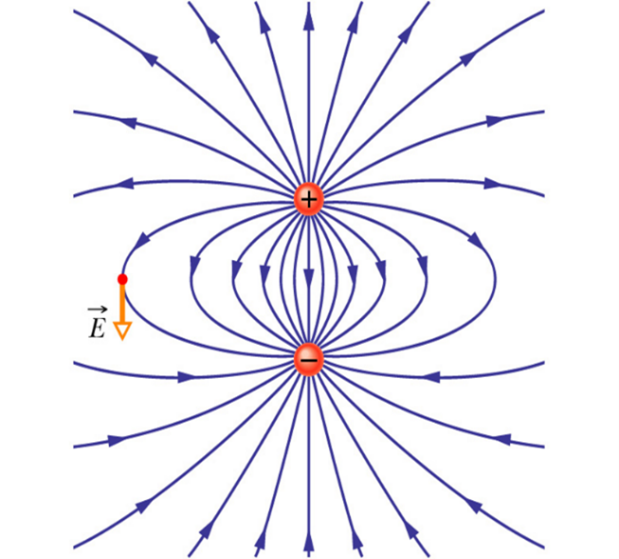
\includegraphics[width=3.125in,height=\textheight]{Figures/dipole_field.png}

The vector field for an electric dipole can be calculated by summing the
vector fields due to the two charges.

Let's consider the dipole in the diagram below. The dipole is oriented
along the \(y\)-axis, and we define an arbitrary point \(P\) on the
\(x\)-axis:

\begin{figure}[H]

{\centering 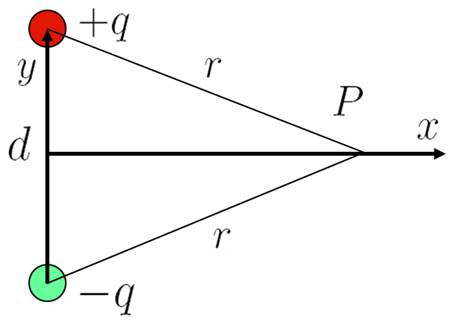
\includegraphics[width=3.125in,height=\textheight]{Figures/dipole_diagram.png}

}

\caption{A dipole represented in the \(x\)-\(y\) plane, where \(d\) is
the distance between the charges.}

\end{figure}%

For dipoles, we define a quantity known as the electric dipole moment,
given by \$\mathrm{\mathbf{p}} = q \mathrm{\mathbf{d}} \$. The electric
dipole moment is the product of the charge \(q\) (pay attention here!
This is the charge on
\bf{one of} the charges, not both added together) and $d$, which is the displacement vector pointing from the negative charge to the positive charge. Note that this is the opposite way to how electric fields are defined, which point from positive to negative charges.  

\begin{figure}[H]

{\centering 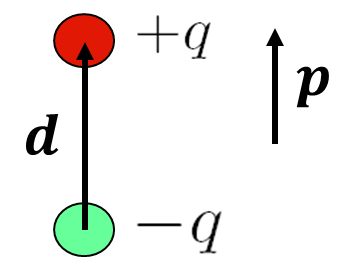
\includegraphics[width=3.125in,height=\textheight]{Figures/dipole_moment.png}

}

\caption{A diagram of an electric dipole, showing the vector quantities
\(\mathrm{\mathbf{d}}\) and \(\mathrm{\mathbf{p}}\), which are the
vector length of the dipole and the dipole moment, respectively.}

\end{figure}%

The field produced by the dipole at point \(P\) on the \(x\)-axis is
given by: \[
\mathrm{\mathbf{E}}= \frac{1}{4\pi \epsilon_0} \frac{qd}{ \left( x^2 \left( \frac{d}{2} \right)^2 \right)^{\frac{3}{2}} }
\]

Does this look familiar? If you attempted the
\bf{post-lecture problem for Lecture 1}, you have actually already calculated the electric field of an electric dipole! The only difference is that in that question you calculated the field at a point on the $z$-axis, but otherwise it should be same mathematical expression. In that problem you were asked to think about the dipole field in different ranges of values of $z$. If we look at the above expression, we can see that in the limit $x >> d$ (in other words, when we are at a distance $x$ from the dipole that is much larger than the size of the dipole $d$) the electric field due to the dipole can be reduced to:
$$
\mathrm{\mathbf{E}}= \frac{1}{4 \pi \epsilon_0} \frac{\mathrm{\mathbf{p}}}{x^3}
$$ 

So the field is very similar to that of a point charge, however it drops
off even faster with distance. If we look at the field lines of the
dipole, we can see how this happens - instead of spreading straight out
from the charges, the field lines bend towards the axis of the dipole,
therefore diverging faster than the point charge case.

\subsection{Energy of a dipole in an external electric
field}\label{energy-of-a-dipole-in-an-external-electric-field}

Now, back to the topic at hand: work and energy.

Consider a dipole that is placed within a uniform electric field. The
force on each charge has magnitude \(qE\), but since these forces are in
opposite directions there is no net force on the dipole. There is
however a torque about the centre of the dipole. See the diagram below
to get a feel for this.

\begin{figure}[H]

{\centering 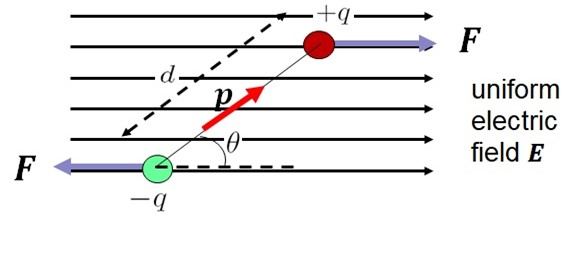
\includegraphics[width=4.16667in,height=\textheight]{Figures/dipole_extE.jpg}

}

\caption{Representation of a dipole placed in an external uniform
electric field. \(\theta\) is the angle the dipole takes to the
direction of the external electric field and \(F\) is the force on each
charge of the dipole due to the external field}

\end{figure}%

The torque about the centre of the dipole is
τ=2Fd2sinθ=qEdsinθ=\textbar p\textbar Esinθ(2.9)(2.9)𝜏=2𝐹𝑑2sin⁡𝜃=𝑞𝐸𝑑sin⁡𝜃=\textbar 𝑝\textbar 𝐸sin⁡𝜃
The direction of the torque is perpendicular to the page, so it can be
represented in vector form as τ=p×E𝜏=𝑝×𝐸. The torque will cause the
dipole to rotate and align itself with the electric field.

We can use the work done by the field to determine what is the minimum
energy configuration (although it should be fairly obvious). The work
done is the integral of the product of the torque and the angle turned
through:
W=∫θθ0\textbar τ\textbar dθ=∫θθ0pEsinθdθ={[}−pEcosθ{]}θθ0(2.10)(2.10)𝑊=∫𝜃0𝜃\textbar 𝜏\textbar d𝜃=∫𝜃0𝜃𝑝𝐸sin⁡𝜃d𝜃={[}−𝑝𝐸cos⁡𝜃{]}𝜃0𝜃
The change in potential energy is ΔU=WΔ𝑈=𝑊,
hence:ΔU=U(θ0)−U(θ)=pE(cosθ0−cosθ)(2.11)(2.11)Δ𝑈=𝑈(𝜃0)−𝑈(𝜃)=𝑝𝐸(cos⁡⁡𝜃0−𝑐𝑜𝑠𝜃)
The zero of potential energy U(θ0)𝑈(𝜃0) can be chosen to be anywhere, so
we can choose it to correspond to θ0=90∘𝜃0=90∘ in which case
U=−pEcosθ𝑈=−𝑝𝐸cos⁡𝜃. This energy can be expressed in vector form as
U=−p⋅E𝑈=−𝑝⋅𝐸. Not surprisingly, the energy is a minimum when the dipole
is aligned with the field at which point the torque will be zero.

\section{Post-lecture problem}\label{post-lecture-problem-2}

As discussed in the lecture, consider a collection of 3 charges that
form 3 sides of a square, as shown:

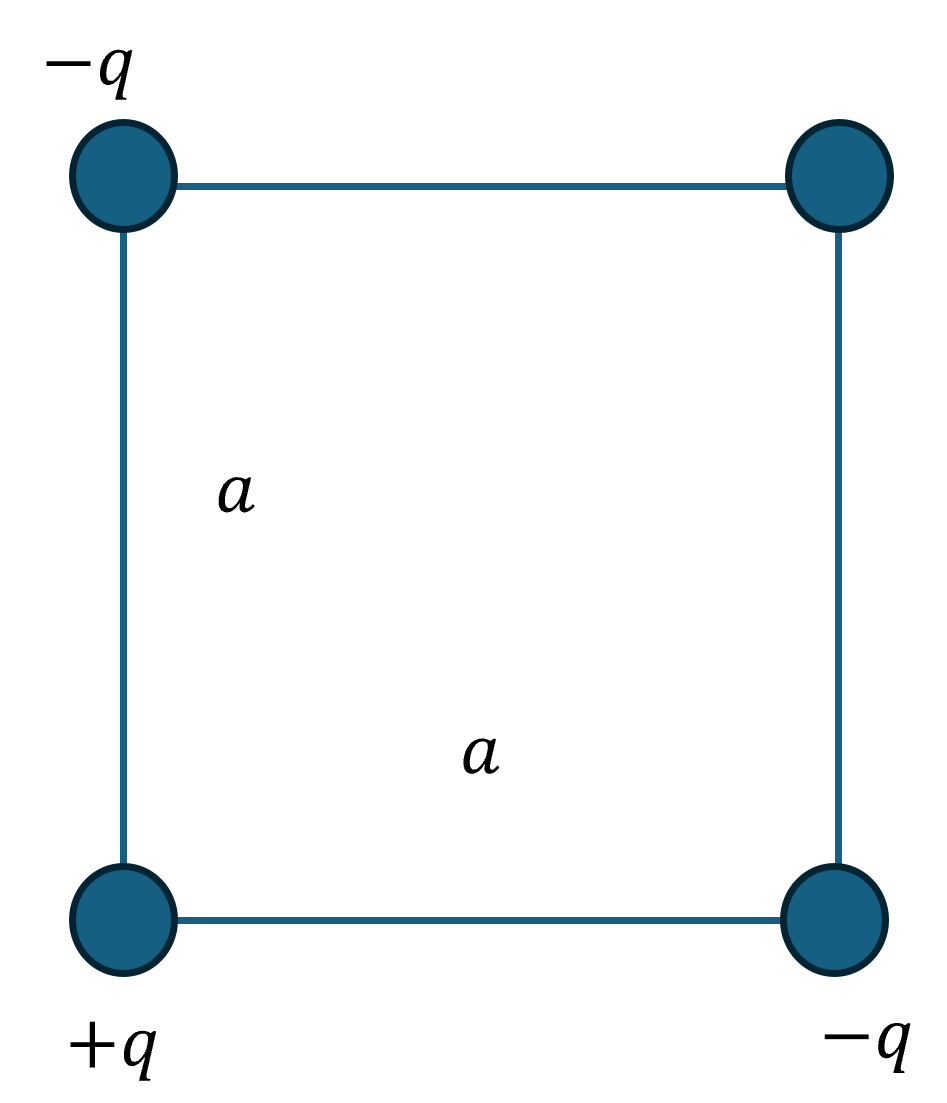
\includegraphics[width=3.125in,height=\textheight]{Figures/L3_3charges.png}

In the lecture, we calculated the amount of work it takes to bring in a
4th charge \(+q\) from far away and place it in the 4th corner of the
square.

\textbf{Q:} Your task is to calculate the total work it takes to
assemble all 4 charges into the square configuration.

\bookmarksetup{startatroot}

\chapter{Magnetic Fields and the Lorentz Force
Law}\label{magnetic-fields-and-the-lorentz-force-law}

\newcommand{\l}{\mathrm{\mathbf{l}}}
\newcommand{\E}{\mathrm{\mathbf{E}}}
\newcommand{\F}{\mathrm{\mathbf{F}}}
\newcommand{\r}{\mathrm{\mathbf{r}}}

\newcommand{\x}{\mathrm{\mathbf{x}}}
\newcommand{\y}{\mathrm{\mathbf{y}}}
\newcommand{\z}{\mathrm{\mathbf{z}}}

\emph{Recommended reading}: Griffiths Section 5.1

\section{Pre-lecture problem}\label{pre-lecture-problem-2}

Griffiths, Problem 5.1

\section{Post-lecture problem}\label{post-lecture-problem-3}

In the lecture we sketched the trajectory of the particle in Example 5.2
at a starting velocity of \((E/B) \hat{\mathrm{\mathbf{y}}}\). We found
that the particle travels in a straight line at a constant speed.

\textbf{Q:} Find and sketch the trajectory of the particle in Example
5.2, if it starts at the origin with velocity: (a)
\((E/2B) \hat{\mathrm{\mathbf{y}}}\) (b)
\((E/B) (\hat{\mathrm{\mathbf{y}}} + \hat{\mathrm{\mathbf{z}}}\))

\bookmarksetup{startatroot}

\chapter{The Biot-Savart Law - Magnetic Fields of
Currents}\label{the-biot-savart-law---magnetic-fields-of-currents}

\newcommand{\l}{\mathrm{\mathbf{l}}}
\newcommand{\E}{\mathrm{\mathbf{E}}}
\newcommand{\F}{\mathrm{\mathbf{F}}}
\newcommand{\r}{\mathrm{\mathbf{r}}}

\newcommand{\x}{\mathrm{\mathbf{x}}}
\newcommand{\y}{\mathrm{\mathbf{y}}}
\newcommand{\z}{\mathrm{\mathbf{z}}}

\emph{Recommended reading}: Griffiths Section 5.2

\emph{A problem to try before attending the lecture}: Force Q, inspired
by p217.

\bookmarksetup{startatroot}

\chapter{Magnetic Vector Potential}\label{magnetic-vector-potential}

\newcommand{\l}{\mathrm{\mathbf{l}}}
\newcommand{\E}{\mathrm{\mathbf{E}}}
\newcommand{\F}{\mathrm{\mathbf{F}}}
\newcommand{\r}{\mathrm{\mathbf{r}}}

\newcommand{\x}{\mathrm{\mathbf{x}}}
\newcommand{\y}{\mathrm{\mathbf{y}}}
\newcommand{\z}{\mathrm{\mathbf{z}}}

\emph{Recommended reading}: Griffiths Section 5.4

\emph{A problem to try before attending the lecture}: Griffiths Problem
1.18

\bookmarksetup{startatroot}

\chapter{Gauss's Law}\label{gausss-law}

\newcommand{\l}{\mathrm{\mathbf{l}}}
\newcommand{\E}{\mathrm{\mathbf{E}}}
\newcommand{\F}{\mathrm{\mathbf{F}}}
\newcommand{\r}{\mathrm{\mathbf{r}}}

\newcommand{\x}{\mathrm{\mathbf{x}}}
\newcommand{\y}{\mathrm{\mathbf{y}}}
\newcommand{\z}{\mathrm{\mathbf{z}}}

\emph{Recommended reading}: Griffiths Section 2.2

\emph{A problem to try before attending the lecture}: Griffiths
{[}insert problem no.{]}

\bookmarksetup{startatroot}

\chapter{Ampere's Law and Solenoids}\label{amperes-law-and-solenoids}

\newcommand{\l}{\mathrm{\mathbf{l}}}
\newcommand{\E}{\mathrm{\mathbf{E}}}
\newcommand{\F}{\mathrm{\mathbf{F}}}
\newcommand{\r}{\mathrm{\mathbf{r}}}

\newcommand{\x}{\mathrm{\mathbf{x}}}
\newcommand{\y}{\mathrm{\mathbf{y}}}
\newcommand{\z}{\mathrm{\mathbf{z}}}

\emph{Recommended reading}: Griffiths Section 5.3

\emph{A problem to try before attending the lecture}: Griffiths
{[}insert problem no.{]}

\bookmarksetup{startatroot}

\chapter{Faraday's Law and Lenz's Law}\label{faradays-law-and-lenzs-law}

\newcommand{\l}{\mathrm{\mathbf{l}}}
\newcommand{\E}{\mathrm{\mathbf{E}}}
\newcommand{\F}{\mathrm{\mathbf{F}}}
\newcommand{\r}{\mathrm{\mathbf{r}}}

\newcommand{\x}{\mathrm{\mathbf{x}}}
\newcommand{\y}{\mathrm{\mathbf{y}}}
\newcommand{\z}{\mathrm{\mathbf{z}}}

\emph{Recommended reading}: Griffiths Section 7.2.1 \& 7.2.2 (for some
bonus reading - check out 7.13)

\emph{A problem to try before attending the lecture}: Griffiths
{[}insert problem no.{]}

\bookmarksetup{startatroot}

\chapter{Maxwell's Equations in Free
Space}\label{maxwells-equations-in-free-space}

\newcommand{\l}{\mathrm{\mathbf{l}}}
\newcommand{\E}{\mathrm{\mathbf{E}}}
\newcommand{\F}{\mathrm{\mathbf{F}}}
\newcommand{\r}{\mathrm{\mathbf{r}}}

\newcommand{\x}{\mathrm{\mathbf{x}}}
\newcommand{\y}{\mathrm{\mathbf{y}}}
\newcommand{\z}{\mathrm{\mathbf{z}}}

\emph{Recommended reading}: Griffiths Section 7.3.1 - 7.3.4

\bookmarksetup{startatroot}

\chapter{Magnetisation and
Polarisation}\label{magnetisation-and-polarisation}

\newcommand{\l}{\mathrm{\mathbf{l}}}
\newcommand{\E}{\mathrm{\mathbf{E}}}
\newcommand{\F}{\mathrm{\mathbf{F}}}
\newcommand{\r}{\mathrm{\mathbf{r}}}

\newcommand{\x}{\mathrm{\mathbf{x}}}
\newcommand{\y}{\mathrm{\mathbf{y}}}
\newcommand{\z}{\mathrm{\mathbf{z}}}

\section{Polarisation}\label{polarisation}

\emph{Recommended reading}: Griffiths Section 4.1 - 4.3

\section{Magnetisation}\label{magnetisation}

\emph{Recommended reading}: Griffiths Section 6.1 - 6.3 (for some bonus
reading - check out 6.4)

\bookmarksetup{startatroot}

\chapter{Maxwell's Equations in
Matter}\label{maxwells-equations-in-matter}

\newcommand{\l}{\mathrm{\mathbf{l}}}
\newcommand{\E}{\mathrm{\mathbf{E}}}
\newcommand{\F}{\mathrm{\mathbf{F}}}
\newcommand{\r}{\mathrm{\mathbf{r}}}

\newcommand{\x}{\mathrm{\mathbf{x}}}
\newcommand{\y}{\mathrm{\mathbf{y}}}
\newcommand{\z}{\mathrm{\mathbf{z}}}

\emph{Recommended reading}: Griffiths Section 7.3.5 - 7.3.6 (for some
bonus reading, check out 7.4)

\bookmarksetup{startatroot}

\chapter{Capacitors and Inductors}\label{capacitors-and-inductors}

\newcommand{\l}{\mathrm{\mathbf{l}}}
\newcommand{\E}{\mathrm{\mathbf{E}}}
\newcommand{\F}{\mathrm{\mathbf{F}}}
\newcommand{\r}{\mathrm{\mathbf{r}}}

\newcommand{\x}{\mathrm{\mathbf{x}}}
\newcommand{\y}{\mathrm{\mathbf{y}}}
\newcommand{\z}{\mathrm{\mathbf{z}}}

\section{Capacitors}\label{capacitors}

\emph{Recommended reading}: Griffiths Section 4.4; Tipler \&
Mosca\ldots{}

\section{Inductors}\label{inductors}

\emph{Recommended reading}: Griffiths Section 7.2.3 \& 7.2.4; Tipler \&
Mosca\ldots{}

\bookmarksetup{startatroot}

\chapter{Circuits}\label{circuits}

\newcommand{\l}{\mathrm{\mathbf{l}}}
\newcommand{\E}{\mathrm{\mathbf{E}}}
\newcommand{\F}{\mathrm{\mathbf{F}}}
\newcommand{\r}{\mathrm{\mathbf{r}}}

\newcommand{\x}{\mathrm{\mathbf{x}}}
\newcommand{\y}{\mathrm{\mathbf{y}}}
\newcommand{\z}{\mathrm{\mathbf{z}}}

\emph{Recommended reading}: Griffiths Section 7.1.1 \& 7.1.2; Tipler \&
Mosca\ldots{}

\bookmarksetup{startatroot}

\chapter{}\label{section}

\newcommand{\l}{\mathrm{\mathbf{l}}}
\newcommand{\E}{\mathrm{\mathbf{E}}}
\newcommand{\F}{\mathrm{\mathbf{F}}}
\newcommand{\r}{\mathrm{\mathbf{r}}}

\newcommand{\x}{\mathrm{\mathbf{x}}}
\newcommand{\y}{\mathrm{\mathbf{y}}}
\newcommand{\z}{\mathrm{\mathbf{z}}}

Impedance

\emph{Recommended reading}: Tipler \& Mosca\ldots{}

\bookmarksetup{startatroot}

\chapter{Summary}\label{summary-2}

In summary, this book has no content whatsoever.

\bookmarksetup{startatroot}

\chapter*{References}\label{references}
\addcontentsline{toc}{chapter}{References}

\markboth{References}{References}

\phantomsection\label{refs}
\begin{CSLReferences}{0}{1}
\end{CSLReferences}



\end{document}
